% Created 2021-09-23 Thu 11:22
% Intended LaTeX compiler: pdflatex
\documentclass[presentation,aspectratio=169]{beamer}
\usepackage[utf8]{inputenc}
\usepackage[T1]{fontenc}
\usepackage{graphicx}
\usepackage{grffile}
\usepackage{longtable}
\usepackage{wrapfig}
\usepackage{rotating}
\usepackage[normalem]{ulem}
\usepackage{amsmath}
\usepackage{textcomp}
\usepackage{amssymb}
\usepackage{capt-of}
\usepackage{hyperref}
\usepackage{khpreamble}
\DeclareMathOperator{\atantwo}{atan2}
\def\ucolor{blue!80!black}
\def\ycolor{green!60!black}
\newcommand*{\incolor}[1]{\textcolor{\ucolor}{#1}}
\newcommand*{\outcolor}[1]{\textcolor{\ycolor}{#1}}
\usetheme{default}
\author{Kjartan Halvorsen}
\date{\today}
\title{Frequency response}
\hypersetup{
 pdfauthor={Kjartan Halvorsen},
 pdftitle={Frequency response},
 pdfkeywords={},
 pdfsubject={},
 pdfcreator={Emacs 26.3 (Org mode 9.4.6)}, 
 pdflang={English}}
\begin{document}

\maketitle

\section{Bode diagram}
\label{sec:org3884654}

\begin{frame}[label={sec:org190f69c}]{Response of LTI systems to sinusoids}
\begin{center}
  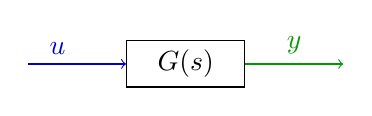
\begin{tikzpicture}[scale = 0.8, node distance=20mm, block/.style={rectangle, draw, minimum width=15mm}, sumnode/.style={circle, draw, inner sep=2pt}]

  \node[coordinate] (refinput) {};
  \node[block, right of=refinput] (motor) {$G(s)$};
  \node[coordinate, right of=motor, node distance=20mm] (output) {};

  \draw[\ucolor, ->] (refinput) -- node[above, pos=0.3] (voltsignal) {$u$} (motor);
  \draw[\ycolor, ->] (motor) -- node[above, pos=0.5] (velsignal) {$y$} (output);
  \end{tikzpicture}
\end{center}

Let \(\incolor{u(t) = \sin\omega_1 t}\). Then, after transients have died out,
\[ \outcolor{y(t)}= \outcolor{|G(\omega_1)| \sin \big( \omega_1 t + \arg G(i\omega_1)\big)}. \]
\end{frame}


\begin{frame}[label={sec:org9403cb3}]{The Bode diagram}
\[ y(t) = \underbrace{|G(i\omega_1)|}_{\text{amplification}} \sin \big( \omega_1 t + \underbrace{\arg G(i\omega_1)}_{\text{phase shift}} \big) \]

The Bode diagram shows the magnitude and phase of the transfer function evaluated on the positive imaginary axis. It thus contains all information about the steady-state response of the system to input signals of different frequency.
\end{frame}


\begin{frame}[label={sec:org8cadac4}]{Specifications on the frequency properties of the closed-loop system}
\begin{center}
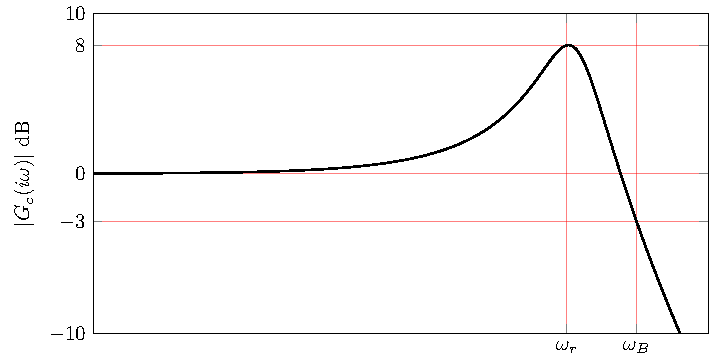
\includegraphics[width=0.899\linewidth]{../../figures/spec-bode-closed-loop-new}
\end{center}
\end{frame}

\begin{frame}[label={sec:orgfc6d2b9}]{Exercise: Reading the Bode diagram}
\begin{center}
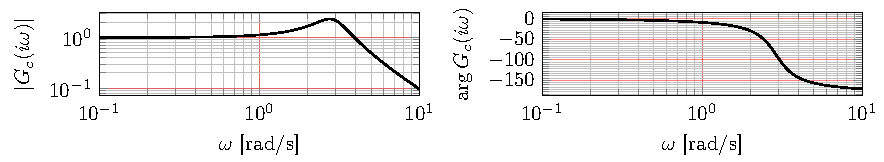
\includegraphics[width=\linewidth]{../../figures/alias-example-bode-GC}
\end{center}
which of the below responses \alert{is not} compatible with the Bode diagram?

\begin{center}
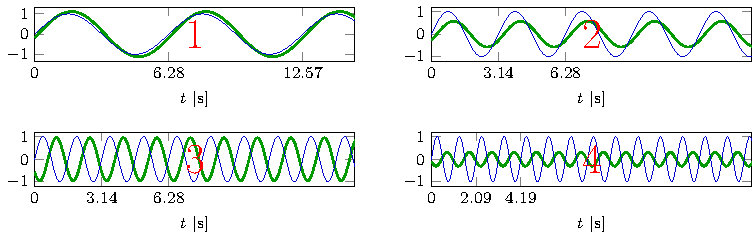
\includegraphics[width=\linewidth]{../../figures/example-bode-GC-timeseries}
\end{center}
\end{frame}

\begin{frame}[label={sec:org61a25fa}]{From loop gain to closed-loop gain}
 \begin{center}
 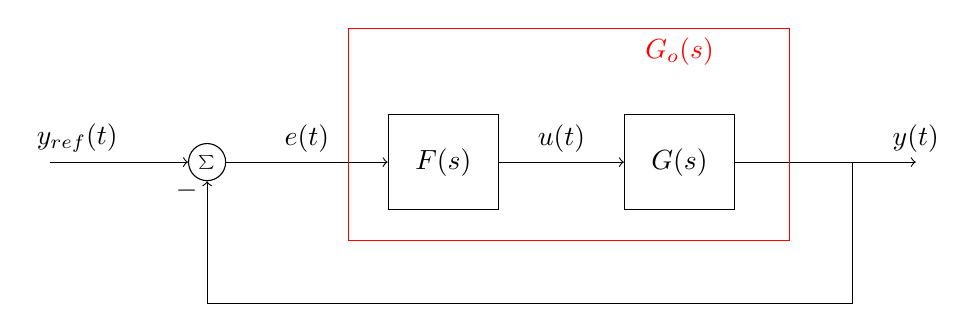
\begin{tikzpicture}
\tikzset{node distance=2cm, 
    block/.style={rectangle, draw, minimum height=12mm, minimum width=14mm},
    sumnode/.style={circle, draw, inner sep=2pt}        
}

  \node[coordinate] (input) {};
  \node[sumnode, right of=input, node distance=20mm] (sum) {\tiny $\sum$};
  \node[block,right of=sum, node distance=30mm] (fb) {$F(s)$};
  \node[block,right of=fb, node distance=30mm] (plant) {$G(s)$};
  \node[coordinate, right of=plant, node distance=30mm] (output) {};
  \node[coordinate, right of=plant, node distance=22mm] (measure) {};
  \draw[->] (input) -- node[above, pos=0.2] {$y_{ref}(t)$} (sum);
  \draw[->] (sum) -- node[above] {$e(t)$} (fb);
  \draw[->] (fb) -- node[above] {$u(t)$} (plant);
  \draw[->] (plant) -- node[at end, above] {$y(t)$} (output);
  \draw[->] (measure) -- ++(0, -18mm) -| (sum) node[left, pos=0.96] {$-$};
  \draw[red] (3.8, -1) rectangle (9.4, 1.7);
  \node[red] at (8, 1.4) {$G_o(s)$};
  \end{tikzpicture}
\end{center}

\[ G_c(i\omega) = \frac{G(i\omega)F(i\omega)}{1 + G(i\omega)F(i\omega)} = \frac{G_o(i\omega)}{1 + G_o(i\omega)} \]
\[ |G_c(i\omega)| = \frac{|G_o(i\omega)|}{|1 + G_o(i\omega)|} = \frac{|G_o(i\omega)|}{|G_o(i\omega) - (-1)|} \]

\pause

\alert{Keep the loop gain \(G_o(i\omega)\) away from -1!} 
\end{frame}





\begin{frame}[label={sec:org8e22d7a}]{If the phase shift is \(\pi\)}
\(G_o(i\omega_1) = -1\), \(|G_o(i\omega_1)| = 1\), \(\arg G_o(i\omega_1) = -\pi\)

\begin{center}
  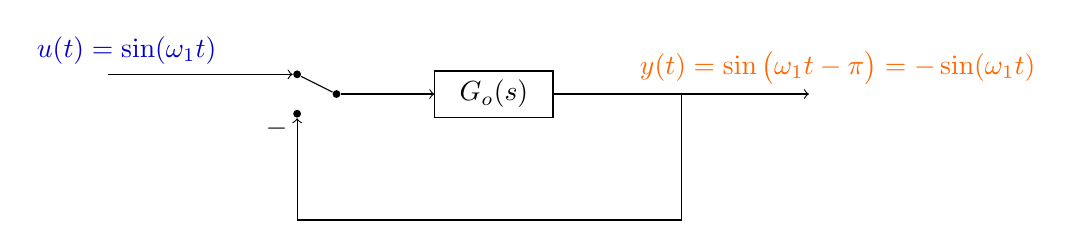
\begin{tikzpicture}[node distance=22mm, block/.style={rectangle, draw, minimum width=15mm}, sumnode/.style={circle, draw, inner sep=2pt}]

    \node[coordinate] (input) {};
    \node[circle, fill, inner sep=1pt, right of=input, node distance=24mm] (sum) {};
    \node[circle, fill, inner sep=1pt, below of=sum, node distance=5mm] (sum2) {};
    \node[coordinate, below of=sum, node distance=2.5mm] (summid) {};
    \node[circle, fill, inner sep=1pt, right of=summid, node distance=5mm] (sum3) {};
    \node[block, right of=sum3, node distance=20mm] (plant)  {$G_o(s)$};
    \node[coordinate, right of=plant, node distance=40mm] (output) {};

    \draw[->] (input) -- node[above, pos=0.1, color=blue!80!black] {$u(t)=\sin(\omega_1 t)$} (sum);
    \draw[->] (plant) -- node[coordinate, pos=0.5] (measure) {} node[above, pos=0.3, anchor=south west, color=orange!80!red] {$y(t)=\sin\big(\omega_1 t -\pi\big) = -\sin(\omega_1 t)$} (output);
    \draw[->] (sum3) -- node[above] {} (plant);
    \draw[->] (measure) -- ++(0,-16mm) -| node[pos=0.95, left] {$-$} (sum2);
    \draw (sum) to (sum3);
  \end{tikzpicture}
\end{center}
\pause
Closed-loop transfer function: \(G_c(s) = \frac{G_o(s)}{1 + G_o(s)}\)
\begin{tcolorbox}
We want \[ 1 + G_o(i\omega) \neq 0, \quad \forall \omega \]
If not, then the closed-loop system will have poles on the imaginary axis (in the s-domain). 
\end{tcolorbox}
\end{frame}

\begin{frame}[label={sec:org4b71672}]{The simplified Nyquist criterion in the s-plane}
\begin{center}
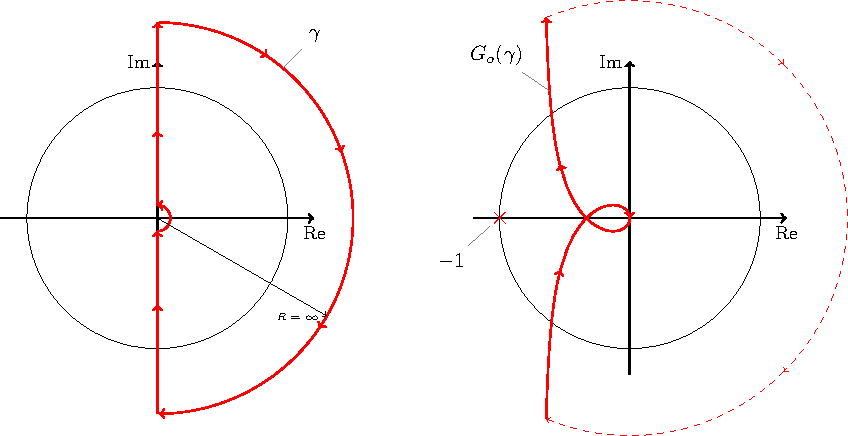
\includegraphics[width=0.65\linewidth]{../../figures/implane-nyquist-contour-map}
\end{center}
\begin{tcolorbox}
If the open-loop system (the loop gain) is not unstable, i.e. $G_o(s)$ has no poles in the right-half plane, then the closed-loop system will be stable if the Nyquist curve \textbf{do not encircle the point \(s=-1\)}. The point $s=-1$ should stay on the left side of the Nyquist curve when we go along the curve from low to high frequencies.
\end{tcolorbox}
\end{frame}

\begin{frame}[label={sec:org26073e1}]{Stability margins}
\begin{center}
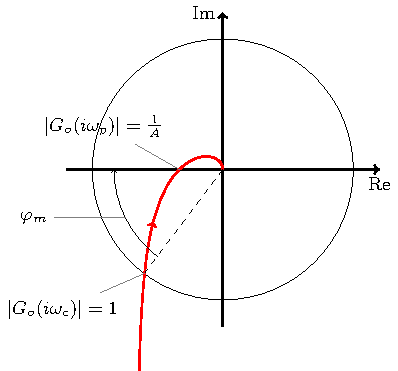
\includegraphics[width=0.38\linewidth]{../../figures/implane-nyquist-margins}
\end{center}
\begin{itemize}
\item Cross-over frequency: The frequency \(\omega_c\) for which \(|G_o(i\omega)| = 1\).
\item Phase margin: The angle \(\varphi_m\) to the negative real axis for the point where the Nyquist curve intersects the unit circle. \[\varphi_m = \arg G_o(i\omega_c) - (-180\degree) = \arg G_o(i\omega_c) + 180\degree\]
\end{itemize}
\end{frame}
\begin{frame}[label={sec:org32b0f3b}]{Stability margins}
\begin{center}
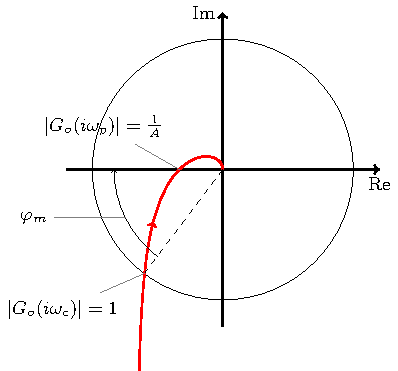
\includegraphics[width=0.38\linewidth]{../../figures/implane-nyquist-margins}
\end{center}
\begin{itemize}
\item phase-cross-over frequency: The frequency \(\omega_p\) for which \(\arg G_o(i\omega) = -180\degree\).
\item Gain margin: The gain \(K=A\) that would make the Nyquist curve of \(KG_o(i\omega h)\) go through the point \(-1 + i0\). This means that \[ |G_o(i\omega_p h| = \frac{1}{A}. \]
\end{itemize}
\end{frame}




\section{Freq-domain specs}
\label{sec:org4f6733a}
\begin{frame}[label={sec:orgd4d0bfd}]{How to achieve the frequency-domain specifications}
\[G_c(i\omega) = \frac{ G_o(i\omega)}{1 + G_o(i\omega)}\]

\alert{Activity}
If \(Go(i\omega) = -0.5\) what is \(|G_c(i\omega)|\)?
If \(Go(i\omega) = -i\) what is \(|G_c(i\omega)|\)?
\end{frame}


\begin{frame}[label={sec:orga286b7d}]{How to achieve the frequency-domain specifications}
\begin{columns}
\begin{column}{0.28\columnwidth}
\[G_c(i\omega) = \frac{ G_o(i\omega)}{1 + G_o(i\omega)}\]

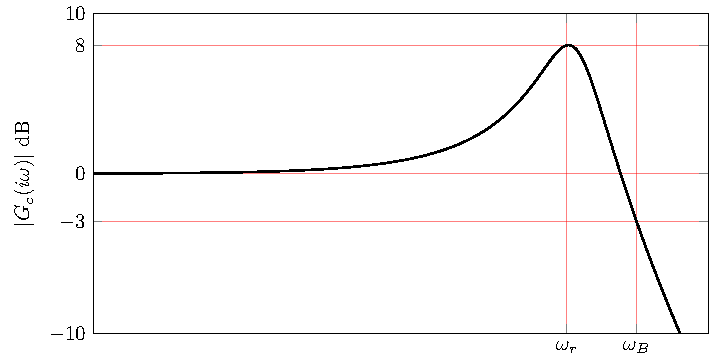
\includegraphics[width=1.1\linewidth]{../../figures/spec-bode-closed-loop-new}

Which of the Bode plots to the right shows the correct loop gain \(G_o(i\omega)\)?
\end{column}

\begin{column}{0.72\columnwidth}
\begin{center}
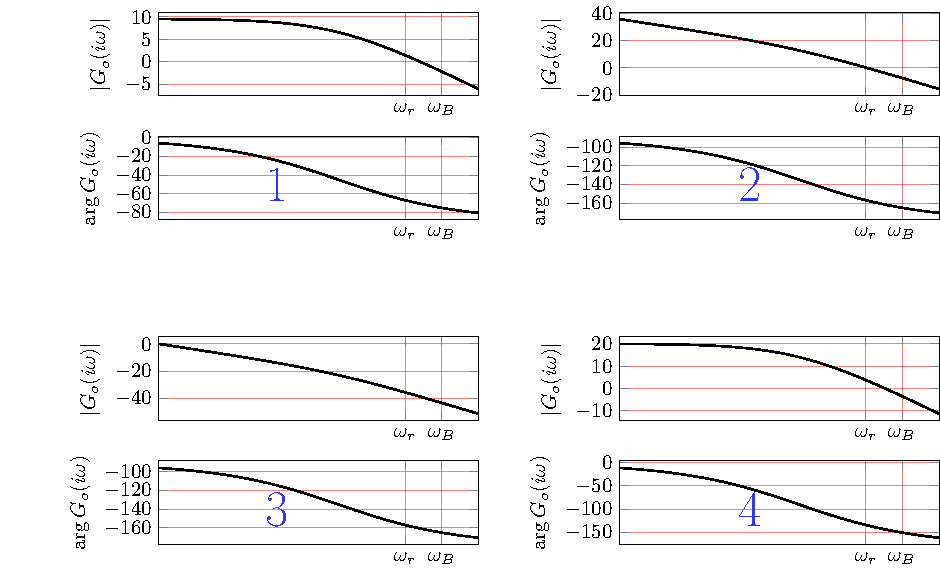
\includegraphics[width=1.02\linewidth]{../../figures/spec-bode-open-loop-new}
\end{center}
\end{column}
\end{columns}
\end{frame}




\begin{frame}[label={sec:org004fad7}]{How to achieve the frequency-domain specifications}
\end{frame}

\begin{frame}[label={sec:orge655a4e}]{Stability margins excercise}
\begin{center}
  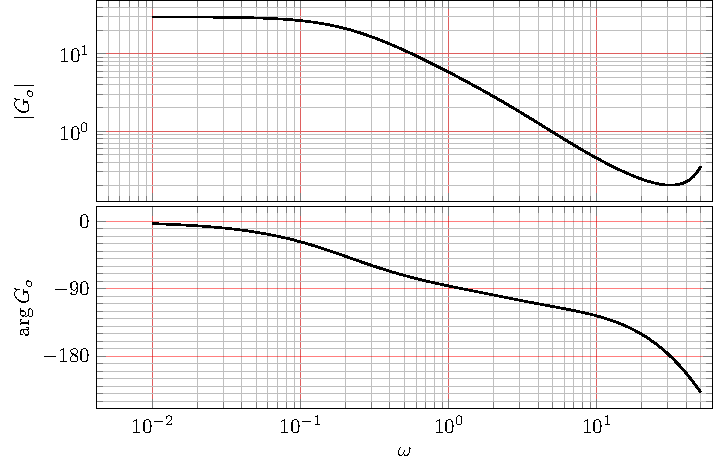
\includegraphics[width=.8\linewidth]{../../figures/bode-example-margin2.pdf}
\end{center}

\alert{Activity} Determine the cross-over frequency \(\omega_c\), the phase cross-over frequency \(\omega_p\), the phase margin and the amplitude margin. 
\end{frame}
\end{document}